\newcommand{\mytwocolumn}[3]{
    \begin{columns}[t,onlytextwidth]
        \begin{column}{#1\textwidth}
            #2
        \end{column}
        \begin{column}{\dimexpr\textwidth-(#1\textwidth)}
            #3
        \end{column}
    \end{columns}
}
\newcolumntype{C}{>{\centering\arraybackslash}X}

\section{Intro}

\begin{frame}{Disclaimer}
    \mytwocolumn{0.55}{
        \begin{wideitemize}
            \item The scope of this project is \emph{\Large huge!}
            \item 8,500 lines of code over 146 files (not including comments, blank space, libraries)
            \item I can't talk about everything interesting in 15 minutes.
            \item This is going to be a whistle-stop tour of the best bits.
            \item Ask me anything after the presentation and I can talk your ear off.
        \end{wideitemize}
    }{
    \vspace{-1.3em}
    \bgroup\begin{table}[t]
        \centering
        {\scriptsize
        \def\arraystretch{2}%  1 is the default, change whatever you need
        \begin{tabularx}{\textwidth}{|CC|}
            \hline
            Timestep calculations & Agnostic sim runners\\
            CUDA Unified Memory & Origin-aware pointers \\
            Parallel Reductions & CUDA Graphs \\
            \texttt{const \_\_restrict\_\_} & Frame allocation \\
            Image Layout Transfers & Vulkan Memory Model \\
            CUDA Warps & Push Constants \\
            Specialization Constants & Indirect Dispatch/Draw \\
            Indexed Rendering & Semaphores \\
            Fences & Vulkan Memory Allocation \\
            Memory Alignment & Atomic Variables \\
            \multicolumn{2}{|c|}{and more!} \\
            \hline
        \end{tabularx}
        }
        \caption{Interesting things I could talk about}
    \end{table}\egroup
    }
\end{frame}

\begin{frame}{CFD, Simulations, and High-Speeds}
    \begin{wideitemize}
        \item Equations modelling real-world phenomena have been around for centuries.
        \item Computational Fluid Dynamics programs (CFD) solve the Navier-Stokes equations to simulate fluid flow.
        \item Used in many fields:
        \begin{wideitemize}
            % \item Weather Simulation\todocite{https://www.futurelearn.com/info/courses/supercomputing/0/steps/24057}
            \item Aerodynamics \parencite{jameson2002}
            \item Fire Spread Modelling \parencite{Sullivan_2009}
            \item Entertainment Industry \parencite{article:FluidDynamicsOnBigScreen,paper:GameFluidSummary:medveckyreal}
        \end{wideitemize}
        \item Generally \textbf{interactive speeds} and \textbf{precise simulation} not pursued together.
    \end{wideitemize}
\end{frame}

\begin{frame}{Project Motivation}
    \begin{wideitemize}
        \item CS257 coursework presented a fluid simulation from \parencite{book:griebel1998numerical}, tasked students with optimizing it for a 6-core CPU.
        \item My solution \parencite{modules:aca257submission} ran 64x faster than the original, and 7.9x faster than real-time, on the given input data.
        \item But the simulation was still limited:
        \begin{wideitemize}
            \normalsize
            \item We were prevented from running it on a GPU for greater speedups.
            \item Results could only be visualized after the fact, even though it was fast enough to render in real time.
        \end{wideitemize}
    \end{wideitemize}
\end{frame}

\begin{frame}{Project Goals/Achievements}
    \begin{center}
        {
        \LARGE
        \textbf{Port the simulation to the GPU.}\\
        \vspace{1em}
        \textbf{Exploit the speedup to improve accuracy and increase sim resolution.}\\
        \vspace{1em}
        \textbf{Intuitively visualize the simulation in real time.\footnote{Use games industry techniques for efficient rendering.}}
        }
        
        %\footnote{Specifically a `tightly-coupled in-situ visualization'\todocite{tightly-coupled in-situ}} in Vulkan
        
        \vfill\null
        {\Large All goals were achieved!}
        
        \vfill\null
        
        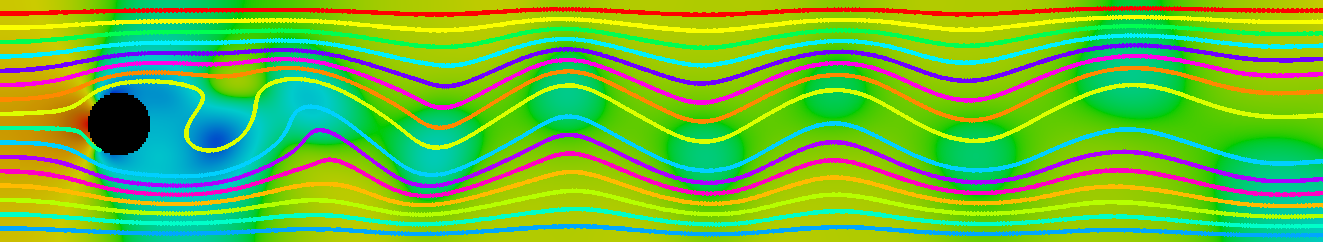
\includegraphics[width=0.7\textwidth]{Presentation/images/viz_particles.png}
        % \begin{tabularx}{\textwidth}{CCC}
        %     \todomark{Figures for speedup} & \todomark{example accuracy} & \todomark{Visualization example} \\
        % \end{tabularx}
    \end{center}
    % \begin{enumerate}
    %     \item Port the simulation to the GPU without significant loss of accuracy.
    %     \item Increase the simulation accuracy.
    %     \item 
    % \end{enumerate}
\end{frame}

% CFDs & Simulation
% - Modelling natural phenomena has been around for ages (Navier-Stokes equations from XX years ago).
% - CFDs are programs that compute results for Navier-Stokes to simulate how fluid moves.
% - Variety of uses
% - generally not required to be at interacive speeds.
%   - when you do, you don't integrate precisely "The model  would  not  be  accurate  enoughfor most engineering applications" [Stam99]

% Vizualization
% Another important property is visualizing the outputs of a simulation.
% Fluid visualization has stagnated - noticed in 2004, still the case today.
% current methods used in Autodesk CFD date back to XX years ago.
% even methods used for viz are getting old
% VTK still uses OpenGL 2 from 2004.

% \begin{frame}{Visualization}
    
% \end{frame}

% Motivation
% ACA coursework last year was to optimize a fluid simulation.
% I optimized it from X to Y, top in class
% But we can go faster
%    - GPU
% and we can visualize it better
%    - in-situ
%    - viz will need to be fast if we're keeping the simulation fast.
%    - use games background, real-time-rendering techniques.
%    - focus on intuive viz